\chapter{Data Samples}
\label{sec:DataSamples}

The data samples is the actual information about collisions taken from the detector. This information is divided into periods, runs and luminosity blocks (LB). The luminosity block is the smallest of the three, it's duration is decided by the ATLAS central trigger processor, and usually is one minute. The data taken within one LB is considered to have constant luminosity, which is calculated separately in stored in the luminosity database. The run represents the data taken during one beam injection. The period is a group of runs with the same detector properties. Each period represents different setup of the detector and/or triggers.

In 2011 there were 13 periods from A to M. Periods A and C were not physical runs, and the period B had only \ensuremath{16.98\,\mathrm{pb}^{-1}} worth of data while having different conditions from other runs and thus was excluded from the analysis.

During some of the runs there were discovered problems with the detector or with the triggers, which compromised the data. Such runs should be excluded from the analysis, and it is done using the good run list (GRL) which lists all the runs and LBs which should be used. In this analysis the common GRL of the WZ group\\
(\texttt{\footnotesize data11\_7TeV.periodAllYear\_DetStatus-v36-pro10\_CoolRunQuery-00-04-08\_WZjets\_allchannels\_DtoM.xml}) was used.

The total luminosity for all the data used in the analysis was calculated by summing the luminosity from all LBs and equals \ensuremath{4.58\,\mathrm{fb}^{-1}} with a systematic uncertainty of $1.8\%$~\cite{lib:lumi}. The timeline of data collection can be seen on Fig.~\ref{fig:data}.

\begin{figure}
\center{
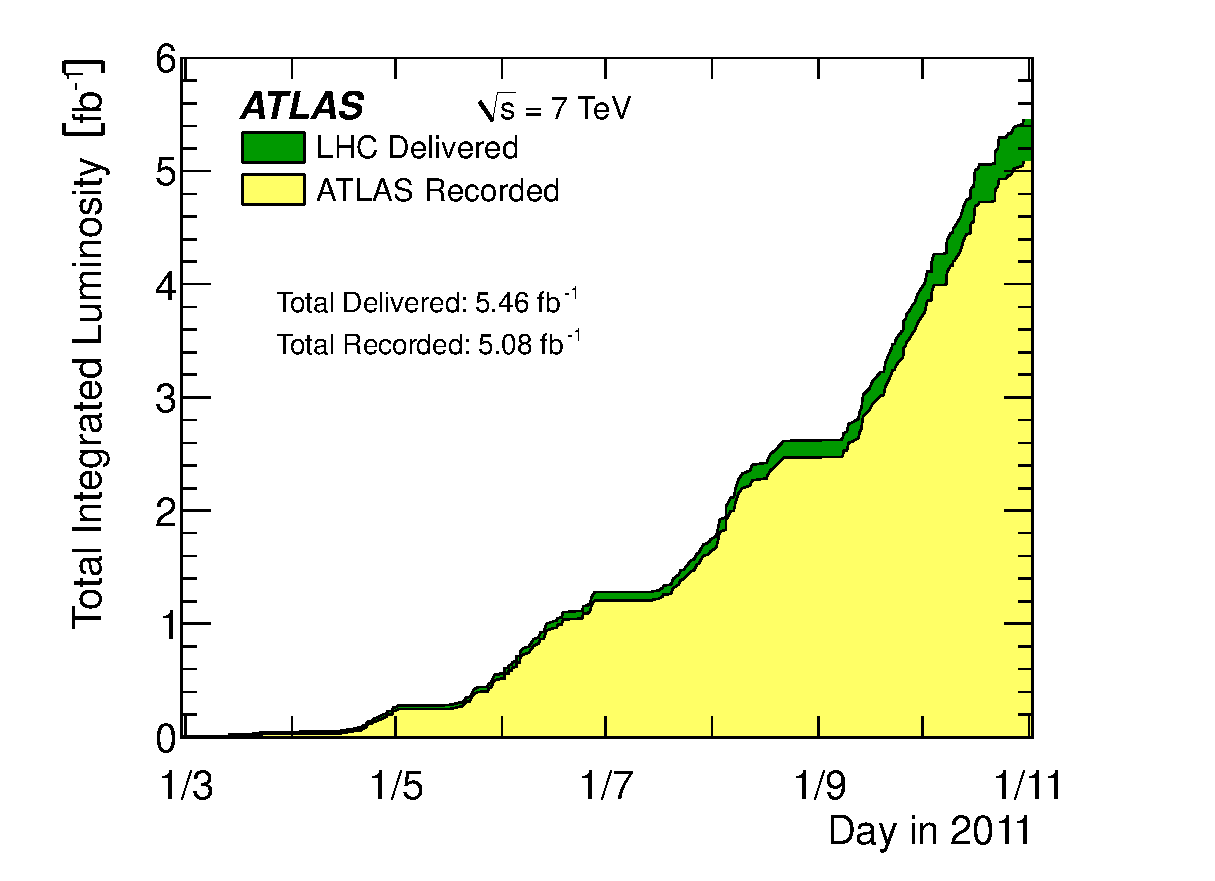
\includegraphics[width=1.0\textwidth]{figures/DATA_lumi.eps}
\caption{The integrated luminosity recorded by the ATLAS detector during 2011.}
\label{fig:data}}
\end{figure}


\begin{table}
\centering
\begin{tabular}{ c | cccl } \hline\hline
Period & Run Range & Lumi [$\rm pb^{-1}$] & Max Lumi $\rm [cm^{-2}s^{-1}]$ & Default SE trigger \\ \hline
D & 179710-180481 & $178.816$ & $6.65\times10^{32}$ & EF\_e20\_medium \\
E & 180614-180776 & $50.176$  & $8.37\times10^{32}$ & EF\_e20\_medium \\
F & 182013-182519 & $152.187$ & $1.11\times10^{33}$ & EF\_e20\_medium \\
G & 182726-183462 & $560.837$ & $1.27\times10^{33}$ & EF\_e20\_medium \\
H & 183544-184169 & $278.271$ & $1.27\times10^{33}$ & EF\_e20\_medium \\
I & 185353-186493 & $399.205$ & $1.90\times10^{33}$ & EF\_e20\_medium \\
J & 186516-186755 & $232.931$ & $2.02\times10^{33}$ & EF\_e20\_medium \\
K & 186873-187815 & $660.211$ & $2.35\times10^{33}$ & EF\_e22\_medium \\
L & 188902-190343 & $1568.848$ & $3.28\times10^{33}$ & EF\_e22vh\_medium1 \\
M & 190503-191933 & $1121.768$ & $3.61\times10^{33}$ & EF\_e22vh\_medium1 \\
\hline
\end{tabular}
\caption{The list of 2011 ATLAS data periods used in the Z analysis.}
\label{tab:data}
\end{table}
